\newpage

\section{Metodología}

La presente sección detalla la secuencia de desarrollo de la solución propuesta, partiendo del análisis del problema hasta su implementación como prueba de concepto (PoC). Se presenta además un flujograma del algoritmo, la arquitectura conceptual del sistema y los aspectos técnicos empleados en la validación de los resultados.

\subsection{Etapas del Desarrollo}

El desarrollo del sistema se dividió en las siguientes etapas:

\begin{enumerate}
    \item \textbf{Análisis del problema}: Se identificaron las principales dificultades en la asignación de tareas en entornos ágiles, especialmente bajo restricciones de habilidades, dependencias y tiempos.
    \item \textbf{Modelado}: Se definieron entidades clave como \textit{tareas}, \textit{desarrolladores}, sus atributos y relaciones. Se eligió el algoritmo genético como técnica de resolución.
    \item \textbf{Diseño e implementación}: Se programó el algoritmo genético en Python, integrando módulos para evaluación de soluciones (fitness), selección por torneo, cruza (crossover) y mutación. También se desarrolló un backend con Flask y un frontend con React.
    \item \textbf{Validación}: Se ejecutaron simulaciones con datos ficticios para analizar la efectividad del sistema bajo distintas configuraciones.
\end{enumerate}

\begin{figure}[htbp]
    \centering
    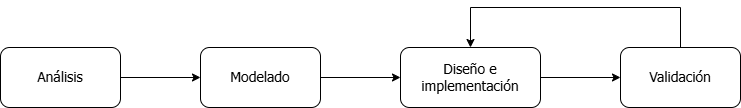
\includegraphics[width=12cm]{imagenes/metodo-secuencia.png}
    \caption{Resumen visual de las etapas del desarrollo del sistema.}
    \label{fig:metodologia}
\end{figure}

\newpage

\subsection{Flujograma del Algoritmo}

La Figura~\ref{fig:flujo} muestra un flujograma general del proceso evolutivo del algoritmo genético implementado.

\begin{figure}[htbp]
    \centering
    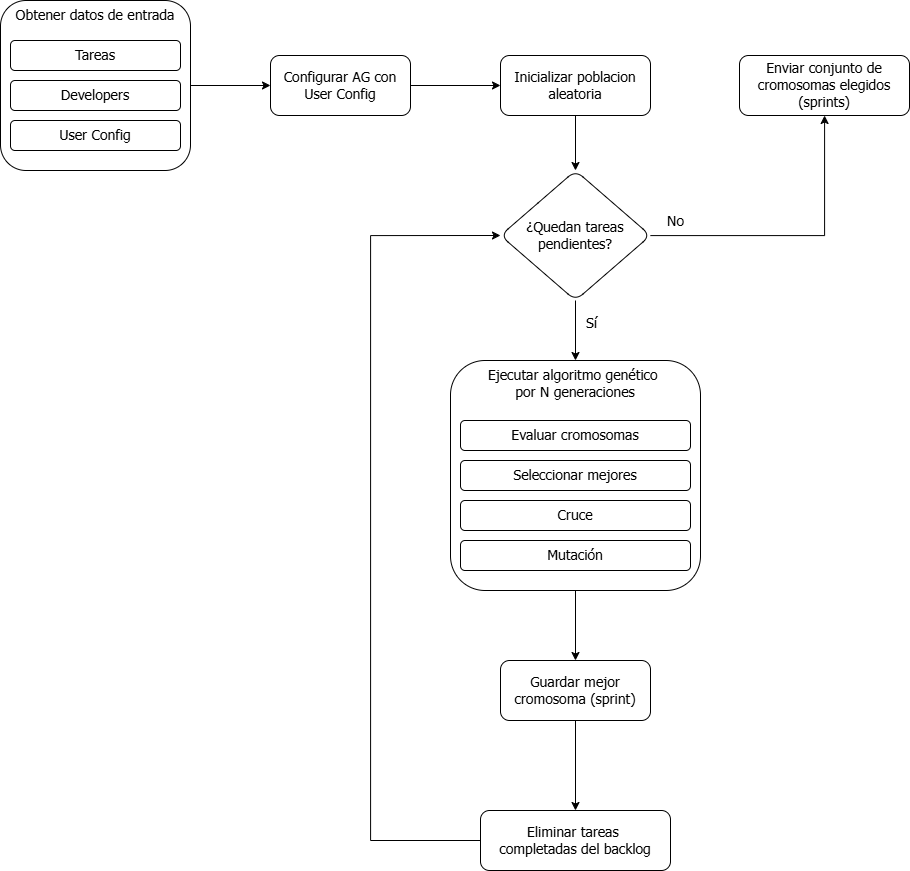
\includegraphics[width=0.8\textwidth]{imagenes/metodo-flow.png}
    \caption{Flujograma general del algoritmo genético}
    \label{fig:flujo}
\end{figure}

\subsection{Arquitectura del Sistema}

La arquitectura general del sistema sigue un modelo cliente-servidor, compuesto por tres capas principales: el frontend, la API backend y el módulo del algoritmo genético. Cada componente cumple un rol específico y se comunican entre sí mediante peticiones HTTP.

\begin{itemize}
    \item \textbf{Frontend}: Desarrollado con React y Vite, es la interfaz gráfica con la que el usuario interactúa para configurar parámetros del algoritmo y visualizar los resultados.
    \item \textbf{Backend/API}: Implementado con Flask en Python, actúa como intermediario entre el frontend y el algoritmo genético. Recibe las configuraciones del usuario y retorna los sprints generados.
    \item \textbf{Algoritmo Genético}: Encapsulado en el backend, este componente ejecuta la lógica evolutiva: inicialización de población, evaluación, selección, cruza, mutación y generación de nuevos sprints.
\end{itemize}

El siguiente esquema resume la interacción entre componentes:

\begin{figure}[htbp]
    \centering
    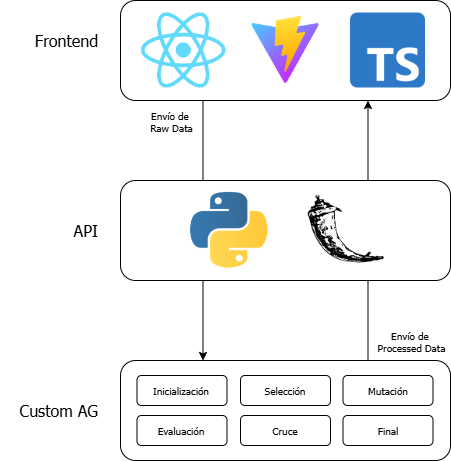
\includegraphics[width=12cm]{imagenes/metodo-arqui.png}
    \caption{Arquitectura general del sistema.}
    \label{fig:arquitectura}
\end{figure}

\subsection{Validación mediante Pruebas Simuladas}

Para validar el sistema, se utilizaron conjuntos de datos representativos de un equipo ágil ficticio. Las simulaciones incluyeron tareas con diferentes niveles de prioridad, complejidad y dependencias, así como desarrolladores con habilidades y capacidades diversas.

Aunque los datos de tareas y desarrolladores eran estáticos (predefinidos en el frontend), se realizaron múltiples experimentos variando los parámetros configurables del algoritmo genético (como el tamaño de la población, la tasa de mutación, la cantidad de generaciones, los pesos de la función objetivo, etc.). Esto permitió analizar el comportamiento del sistema bajo distintas condiciones.

Además, el desarrollo del algoritmo se llevó a cabo de forma incremental y validada. Cada módulo del algoritmo genético —como la inicialización, evaluación, selección por torneo, cruza y mutación— fue implementado y probado por separado. Posteriormente, se integraron de forma progresiva hasta alcanzar la versión final con todas las restricciones consideradas: cumplimiento de dependencias, balance de carga, coincidencia de habilidades, y penalización por tareas no asignables o desarrolladores sobrecargados.

Las métricas utilizadas para evaluar la efectividad del sistema incluyeron:

\begin{itemize}
    \item \textbf{Tiempo total estimado del sprint} (\textit{makespan}).
    \item \textbf{Balance de carga} entre desarrolladores.
    \item \textbf{Coincidencia de habilidades} entre tareas y asignados.
    \item \textbf{Cumplimiento de dependencias} entre tareas.
    \item \textbf{Costo estimado} de asignación basado en las horas de cada desarrollador.
\end{itemize}

Los resultados obtenidos demuestran que el sistema logra generar sprints viables y balanceados en tiempos razonables, y que responde de manera coherente ante variaciones en los parámetros evolutivos.

\subsection{Herramientas y Tecnologías Utilizadas}

El desarrollo del sistema se apoyó en una serie de herramientas y tecnologías modernas que facilitaron la implementación modular y colaborativa del proyecto. A continuación se detallan:

\begin{itemize}
    \item \textbf{Lenguajes de programación}: Python para el backend y JavaScript/TypeScript para el frontend.

    \item \textbf{Frameworks y entornos}:
          \begin{itemize}
              \item \textit{Flask} para la creación de la API REST.
              \item \textit{React} y \textit{Vite} para el desarrollo del frontend, con enrutamiento gestionado mediante React Router.
          \end{itemize}

    \item \textbf{Control de versiones}: Git y GitHub fueron utilizados para el seguimiento del desarrollo y la colaboración en equipo.

    \item \textbf{Entorno de desarrollo}: Visual Studio Code fue el editor principal, junto con extensiones y herramientas como Thunder Client para pruebas de API.

    \item \textbf{Diagramación}: Draw.io fue empleado para la elaboración de flujogramas y diagramas de arquitectura.

    \item \textbf{Documentación}: La redacción del informe se realizó utilizando LaTeX, empleando una plantilla compartida mediante GitHub.
\end{itemize}


% \section{Metodología}

% La solución propuesta se desarrolla en etapas que siguen una secuencia lógica de análisis, diseño, implementación y validación. Inicialmente, se definen los parámetros de entrada: tareas, programadores, tiempos estimados y dependencias. Luego, se formula el problema como una función objetivo y se implementa un algoritmo genético con operadores personalizados.

% Se incluye un flujograma general del sistema, así como una arquitectura conceptual que modela la interacción entre módulos. Finalmente, se valida la solución a través de casos simulados.

% \vspace{0.5cm}

% \begin{tcolorbox}[colback=gray!10, colframe=black!30, title={Sugerencias para esta sección}]
%     \begin{itemize}
%         \item Usa un flujograma para mostrar el proceso general (puedes incluirlo más adelante).
%         \item Describe cómo se estructura el algoritmo: población, selección, cruza, mutación, etc.
%         \item Explica cómo se simula el entorno SCRUM para validar resultados.
%         \item Detalla cualquier herramienta o lenguaje usado (Python, etc.).
%     \end{itemize}
% \end{tcolorbox}